\chapter{Onderzoeksopzet}
\label{chap:Onderzoeksopzet}
Voor dit onderzoek wordt de methodiek van \textit{Wat is Onderzoek?} \Parencite{Verhoeven} toegepast. 
Dit hoofdstuk omvangt de ontwerpfase van het onderzoek in de onderzoekscyclus (zie figuur \ref{fig:OntwerpenCyclus}).
Eerst wordt de doelstelling besproken van het onderzoek met daar een bij passende hoofdvraag voor het onderzoek.
Daarna wordt de methodologie beschreven van het onderzoek.

\begin{graphic}
	\vspace{0.2cm}
	\captionsetup{type=figure}
    \caption{Deel 1 Verhoeven ontwerpen afgeleid van \textit{Wat is Onderzoek?}}
	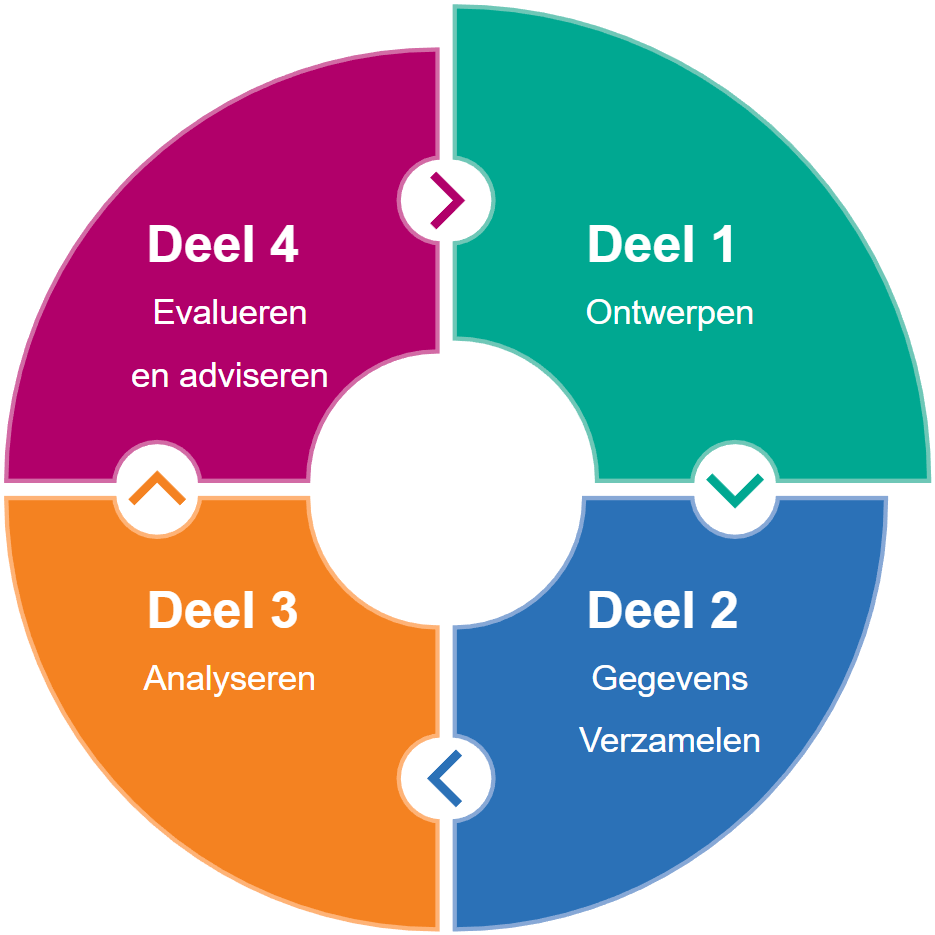
\includegraphics[scale=0.3]{img/OntwerpenCyclus.png}
	\label{fig:OntwerpenCyclus}
	\vspace{0.2cm}
\end{graphic}

\section{Doelstelling}
\label{sec:Doelstelling}
Om het proof of concept te realiseren moet er eerst bekend zijn wat er gemaakt moet worden en voor wie.
Hierom moet er een lijst aan geprioriteerde requirements komen voor 22 november 2023 voor het \qw{het CMS voor iedereen} project.
Deze lijst moet worden samengesteld in samenwerking met de stakeholders. Hierom is de volgende hoofdvraag opgesteld:

\whitespace
\begin{center}
    \textit{\MainQuestion}
\end{center}

\newpage
\section{Methodologie}
In dit hoofdstuk wordt de methodologie van het onderzoek beschreven.
Om een volledig antwoord te kunnen geven op de hoofdvraag, wordt deze vraag opgedeeld in meerdere deelvragen.
Voor het beantwoorden van de verschillende deelvragen wordt er gebruikt gemaakt van de onderzoeksmethoden die beschreven zijn door HBO-I \Parencite{HBO-i-reasearch-methods}.
% \todo[inline]{Dot framework ?}
\subsection{Deelvraag 1: Stakeholders}
Voor het opstellen van de requirements is het belangrijk om te weten voor wie je het maakt.
Daarom is het belangrijk om de stakeholders van het project in beeld te brengen.
Hierom wordt de volgende deelvraag gesteld:

\begin{center}
	\textit{\SubquestionOne}
\end{center}

\whitespace[0.2]
Om deze deelvraag te beantwoorden wordt er een \textbf{stakeholdersanalyse} uitgevoerd.
Dit wordt gedaan door samen met de product owner een \textbf{brainstorm} sessie te houden.
Na deze sessie zullen de stakeholders geprioriteerd worden op basis van belang en invloed op het project.
Tot slot worden de stakeholders weer gegeven in een stakeholders matrix (ook wel een Mendalow matrix genoemd \Parencite{MandelowMatrix})om hun positie weer te geven in het project.
Het resultaat van de deelvraag zou leiden tot een lijst van geprioriteerde stakeholders die gebruikt worden om de andere deelvragen te beantwoorden.
Aan het einde van de stakeholdersanalyse worden de resultaten teruggelegd aan de product owner om de resultaten te valideren.

\todo[inline]{Ja dat is Elsa, zij is gekwalificeerd omdat zij met de kleinste klanten van Snakeware werkt.
Maar wat je al zij volgens mij ben ik de Product owner of heb ik dat verkeerd.}
% \todo[inline]{Resultateren de artifacts benoemen.Mendelow matrix komt uit de lucht vallen}
% \todo[inline]{\textit{Wie is de product owner in deze context? is hij te vertrouwen om gegevens hiervoor te leveren? en waarom?}, bang dat ik te kort kom aan woorden}

\subsection{Deelvraag 2: Architectuur}
Om de huidige problemen van het Snakeware cloud platform in beeld te brengen is het belangrijk dat er gekeken wordt naar de huidige software-architectuur.
Hier uit wordt een lijst met problemen verzameld die de huidige software-architectuur nu heeft.
Daarom is de volgende deelvraag opgesteld:

\begin{center}
	\textit{\SubquestionTwo}
\end{center}

\whitespace[0.2]
Door te onderzoeken hoe de huidige softwarearchitectuur in elkaar zit en onderhouden is kan er een beeld geschetst worden van de huidige problemen met Snakware Cloud.
Hierom is er voor gekozen om gebruik te maken van \textbf{IT architecure sketching} om de huidige softwarearchitectuur in beeld te brengen.
Samen met het R\&D team zal er een sessie gepland worden om de huidige architectuur in beeld te krijgen.
Het resultaat dat uit deze deelvraag komt wordt gebruikt ter ondersteuning van deelvraag 3.
% \todo[inline]{verwachte resultaat?}

\subsection{Deelvraag 3: Knelpunten}
Een van de doelen van het proof of concept is het oplossen van de huiige problemen die de klant en Snakeware nu hebben met het huidige systeem.
Daarom is het belangrijk om de huidige knelpunten van het systeem te inventariseren.
Hierom is de volgende deelvraag gemaakt:

% Omdat een van de doelen van het  proof of concept is het oplossen van de huidige problemen die de klant en Snakeware heeft met het huidige systeem.
% Daarom is het belangrijk om te inventariseren wat de huidige knelpunten zijn van het systeem. 
% Hierom is de volgende deelvraag gemaakt:
%
% Om het systeem te kunnen ontwikkelen moeten er requirements aan het systeem gesteld worden.
% Deze requirements moeten op basis van de eisen en wensen van de stakeholders gemaakt worden.
% Hieruit zal een lijst requirements komen waar mee het systeem gerealiseerd wordt.
% Daarom is de volgende deelvraag gemaakt:
%
\begin{center}
    \textit{\SubquestionThree}
\end{center}

\whitespace[0.2]
Om deze deelvraag te beantwoorden wordt er een semi-gestructureerd \textbf{expertinterview} gehouden.
Binnen Snakeware zijn er meerdere mensen die geschikt zijn om de knelpunten van het Snakeware cloud platform te kunnen aankaarten.
De volgende mensen worden de interviews afgenomen:
\begin{itemize}
    \item[-] Janny Reitsma (Service desk lead?): Reitsma heeft veel inzicht in waar de huidige klanten van snakeware tegen aanlopen.
        Verder krijgt ze alle klachten van de klanten van Snakeware mee en weet ze waar de huidige klanten van Snakeware behoefte aan hebben.
    \item[-] Rob Douma (Product owner van meerdere projecten): Douma werkt aan meerdere projecten als product owner en weet veel van Snakeware cloud.
        Hij heeft veel technische kennis over het platform en kan goed in beeld brengen wat de huidige technische imitaties zijn van het platform.
\end{itemize}

\whitespace
Er is overwogen om Hans Hoomans (CEO) en Johan Nieuwehuis (CTO) te interviewen om de huidige knelpunten in beeld te brengen.
Dit is uiteindelijk niet gedaan vanwege de tijd die beschikbaar is voor het onderzoek.
% Na de expert interviews zal er een taak analyse uitgevoerd worden om de werkwijze van het CMS in beeld te krijgen.
\todo[inline]{Ik weet niet of de titles kloppen van Rob en Janny}

\subsection{Deelvraag 4: Requirements}
Om het systeem te kunnen ontwikkelen moeten er requirements aan het systeem gesteld worden.
Deze requirements moeten op basis van de eisen en wensen van de stakeholders gemaakt worden.
Daarom is de volgende deelvraag gemaakt:

\begin{center}
 \textit{\SubquestionFour}
\end{center}

\whitespace[0.2]
Om deze deelvraag te beantwoorden wordt er gebruik gemaakt van \textbf{explore user requirements}.
De communicatiemethode met de stakeholders wordt bepaald op basis van hun positie binnen het project door middel van de stakeholder matrix.
Voor de sleutelfiguren worden er semigestructureerde \textbf{interviews} gehouden om genoeg vrijheid te geven tijdens de gesprekken om dieper op vragen in te gaan.
% Daarnaast worden er met de geïnteresseerde een \textbf{focus group} gepland om hier met de betrekkende stakeholders meerdere onderwerpen te bespreken die belangrijk zijn voor het project.
% Voor de focus groep zal er gebruik gemaakt worden van een aantal voorbereide vragen om de focus groep in een goede richting te sturen.
Het resultaat van deze deelvraag zou leiden tot een lijst van eisen en wensen die worden vertaald in requirements.
Als de eisen en wensen zijn bepaald door middel van de interviews worden ze genoteerd zodat ze in de volgende deelvraag geprioriteerd kunnen worden.
% Als de eisen en wensen zijn bepaald door middel van de focus group en interviews worden ze genoteerd zodat ze in de volgende deelvraag geprioriteerd kunnen worden.
% \todo[inline]{Verwachte resultaat?}
% Hieruit zal een lijst requirements komen waar mee het systeem gerealiseerd wordt.


\subsection{Deelvraag 5: Prioritering}
Na het opstellen van een lijst met requirements als resultaat van deelvraag 4.
Deze lijst is echter nog niet bruikbaar, aangezien deze niet is geprioriteerd.
Om de prioriteiten van de requirements vast te stellen, wordt de volgende deelvraag geintroduceerd.

\begin{center}
	\textit{\SubquestionFive}
\end{center}

\whitespace[0.2]
Dit wordt gedaan door middel van \textbf{requirements prioritization} zal er verschillende prioriteit niveaus toegekend worden aan de requirements.
Deze niveaus worden in beeld gebracht door middel van MoSCoW-methode \Parencite{MoSCoW}.
%
% tevredenheidsscore [1,2, \dots, 5]
% ontevredenheidscore [1,2 \dots, 5]
% duur (1,2,3,5,8)
% Stakeholder positie [1,2,3,4]

\whitespace
Om de prioritering te bepalen wordt er gebruik gemaakt van een formule (zie formule \ref{eq:prioritization}), in de ze formule wordt de volgnede aspecten in mee genomen.
\begin{enumerate}
	\item[-] tevredenheidsscore (TS) [1,2,\ldots,5]: dit is de waarde die door de stakeholder gegeven wordt als de requirement geimplementeerd wordt
	\item[-] ontevredenheidscore (OS) [1,2,\dots,5]: Dit is de waarde die door de stakeholder gegeven wordt wanneer het niet geimplementeerd wordt.
	\item[-] stakeholder invloed positie (SIP) [1,2,3,4]: Op basis van de stakeholders matrix wordt er een waarde aan een stakeholder groep toegekend 1 voor sleutelfiguren, 2 voor beinvloeder, 3 voor geintreceerde en 4 voor toeschouwer.
	\item[-] duur [1,2,3,5,8]: De duur representeert door een relatief getal om de geschatte tijd om de requirement te implementeren te representeren.
	      De waardes van de duur zijn een verkleinde selectie van Scrum poken \Parencite{ScrumPoker}.
\end{enumerate}
% De prioritering van de requirements wordt berekend door de volgende formule.
%
%
% De prioriteit van de requirements wordt berekend op basis van de invloed en het belang van de stakeholders,
% de tevredenheidsscore [1,2,\ldots,5] bij implementatie, de ontevredenheid score [1,2,\ldots,5] als het niet geïmplementeerd wordt en de duur van de implementatie (1,2,3,5,8) die wordt weer gegeven door een relatief getal.
% De berekening wordt gedaan door middel van de volgende formule:
% \begin{center}

\whitespace
	\begin{equation}
		\label{eq:prioritization}
		Score = SIP + TS - OS + (9 - duur)
	\end{equation}
% \end{center}

\whitespace
nadat er een score is berekend wordt er een prioriteit niveau toegegeven op basis van de MoSCoW methode:

\begin{itemize}
	\item{\makebox[3cm]{Must have:} $x \in \mathbb{R} : 14 \leq x \leq 18$}
	\item{\makebox[3cm]{Should have:} $x \in \mathbb{R} : 14 \leq x \leq 18$}
	\item{\makebox[3cm]{Could have:} $x \in \mathbb{R} : 14 \leq x \leq 18$}
	\item{\makebox[3cm]{Won't have:} $x \in \mathbb{R} : 14 \leq x \leq 18$}
\end{itemize}

\whitespace
De requirement worden vervolgens genoteerd in een gemodificeerde versie van een snow card.
Na het maken van de requirement wordt er terug gekoppeld met de stakeholder om het te verifiëren
als de volledige lijst gemaakt is wordt het gecheckt met de product owner en de bedrijfsbegeleider.
\whitespace
\todo[inline]{Maak fancy snow card en fancy formule en daarna tekst verbeteren scores kloppen ook nog niet want deze moeten besproken worden en eigelijk pas gesteld worden tijden de deelvraag ?}
\todo[inline]{Artifacts en formule}



% \section{Onderzoeksvragen}
Text text text\\
\textbf{Hoofdvraag:} \textit{\MainQuestion} \\

Text text text\\

\textbf{Deelvraag 1:} \textit{\SubquestionOne}\\

\textbf{Deelvraag 2:} \textit{\SubquestionTwo} \\

\textbf{Deelvraag 3:} \textit{\SubquestionThree} \\
text\\ 
\textbf{Deelvraag 4:} \textit{\SubquestionFour} \\

\textbf{Deelvraag 5:} \textit{\SubquestionFive} \\

% \newpage
% \section{Onderzoeksmethoden}
onderzoeksmethoden\\
\textbf{Deelvraag 1:} \textit{\SubquestionOne}\\

\textbf{Deelvraag 2:} \textit{\SubquestionTwo} \\

\textbf{Deelvraag 3:} \textit{\SubquestionThree} \\
text\\ 
\textbf{Deelvraag 4:} \textit{\SubquestionFour} \\

\textbf{Deelvraag 5:} \textit{\SubquestionFive} \\

